\documentclass{article}
\usepackage{nips13submit_e,times}
\usepackage[utf8x]{inputenc}
\usepackage{amsfonts}
\usepackage{indentfirst}
\usepackage{hyperref}
\usepackage{graphicx}
\usepackage{enumerate}
\usepackage{amsmath}
\usepackage{subfigure} 
\usepackage{amsopn}
\title{Project-I by group TORONTO}
\author{Michalina Pacholska \And Jakub Sygnowski}
\nipsfinalcopy
\begin{document}
\maketitle
\begin{abstract}
    This raport describes our work on first project done for Machine Learning class at EPFL in Fall 2014. We were given two synthetic datasets - a regression and a classification one and used methods learnt in the class to train few models and predict regression and classification outcome for the test data we got. 
\end{abstract}
\begin{section}{Text structure - usunac?}
As the two tasks - regression and classification are independent of each other, we split the raport into two sections.
\end{section}

\begin{section}{Classification}
\begin{subsection}{Data preparation}
Our dataset consists of train data, for which we have both input variables $X$ and output $y$ and test data, for which we observe only $X$ and have to produce our predictions and approximation of certainity.

Both original train and test data sets included $N=1500$ samples, each has $33$ dimensions. All except $3$-rd input variable are continuous, $3$-rd is a binary one. Our $X_train$ matrix has full-rank, so we don't expect one input variable to be a linear function of other ones. 
Data we got was not normalized, as shown in figure \ref{fig:boxplotBefore}, so we decided to normalize it. We also normalized test data using same means and standard deviations. After that, we randomly a subset of $N=70$ data samples to leave it aside and use it at the end to estimate RSME error without being biased because of using cross-validation. 

Figure \ref{fig:boxplotBefore} shows also that our data is not free of outliers. We decided to remove from dataset all samples that have absolute value of any input variable $\ge 5$ standard deviations of this input variable.

After these procedures, we end up with normalized data shown on figure \ref{fig:boxplotAfter}. There was $N=1284$ data samples left available to train our model.

\begin{figure}[!h]
\center
\subfigure[Boxplot of original input data $\mathbf{X}$. Data is not centered and therefore we normalize it.]{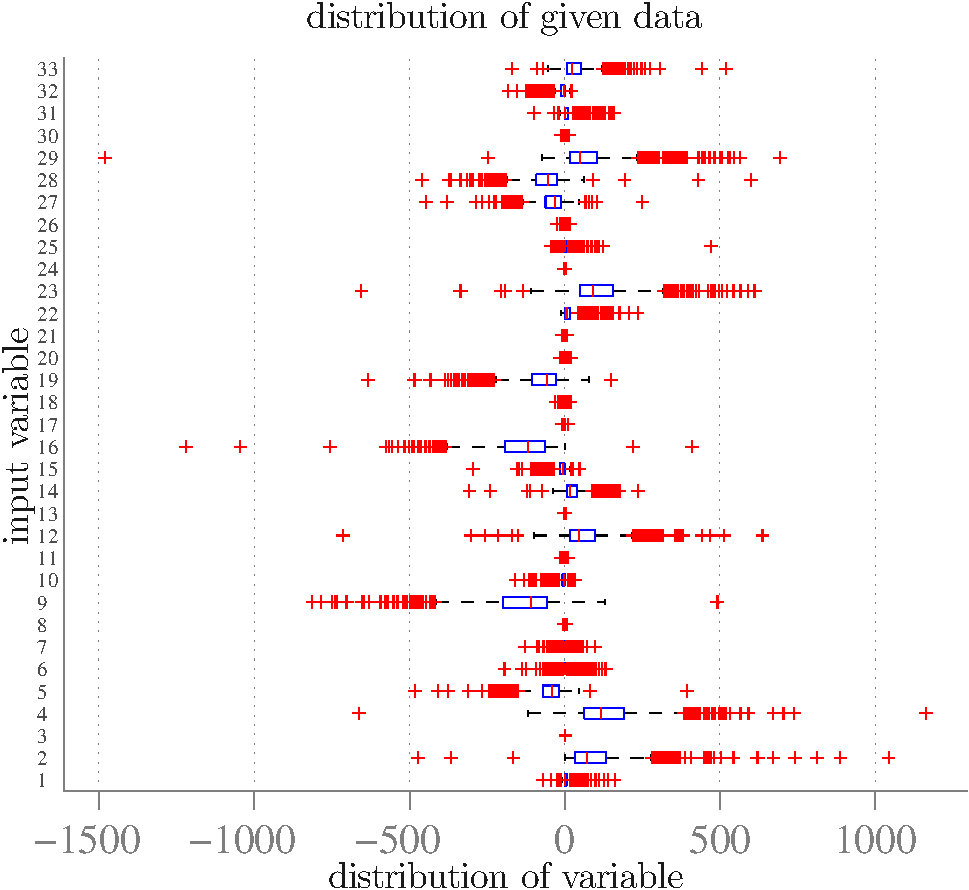
\includegraphics[width=2.5in]{../figures/boxplot_before-crop.pdf} \label{fig:boxplotBefore}}
\hfill
\subfigure[Boxplot of input data after normalization and removing outliers.]{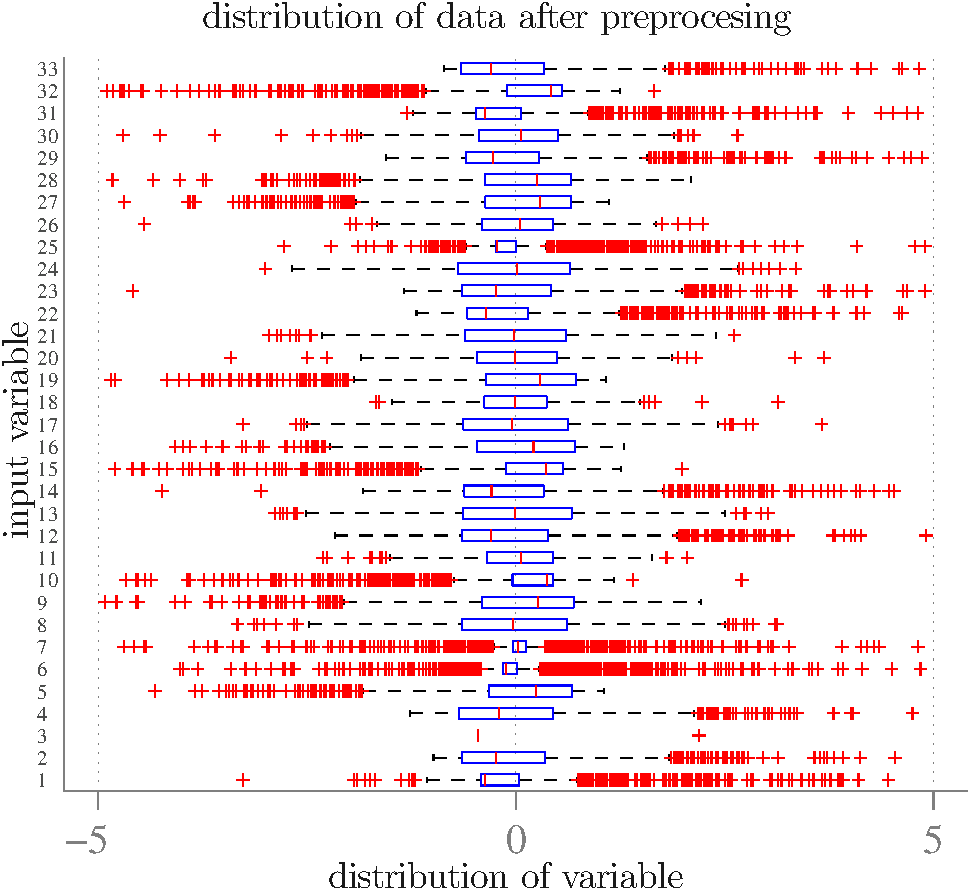
\includegraphics[width=2.5in]{../figures/boxplot_after-crop.pdf} \label{fig:boxplotAfter}}
\caption{}
\end{figure}

\end{subsection}
\begin{subsection}{Data analysis}
We investigated correlation between different input variables and an output variable and amongst input variables themselves. Figure \ref{fig:correlation} shows that some variables are clearly more correlated to the output then the others. While building models we sometimes tried to create them only using few most correlated variables. On the other hand, we found no interesting correlation between input variables. We also tried to apply PCA to extract principal components of the data, but we found that particular principal components are not so well correlated with output variable, so we abandoned this path and did not use PCA later.

\begin{figure}[!t]
\center
\subfigure[Correlation between input variables and output variable. Some variables have much bigger correlation to the output variable than the others.]{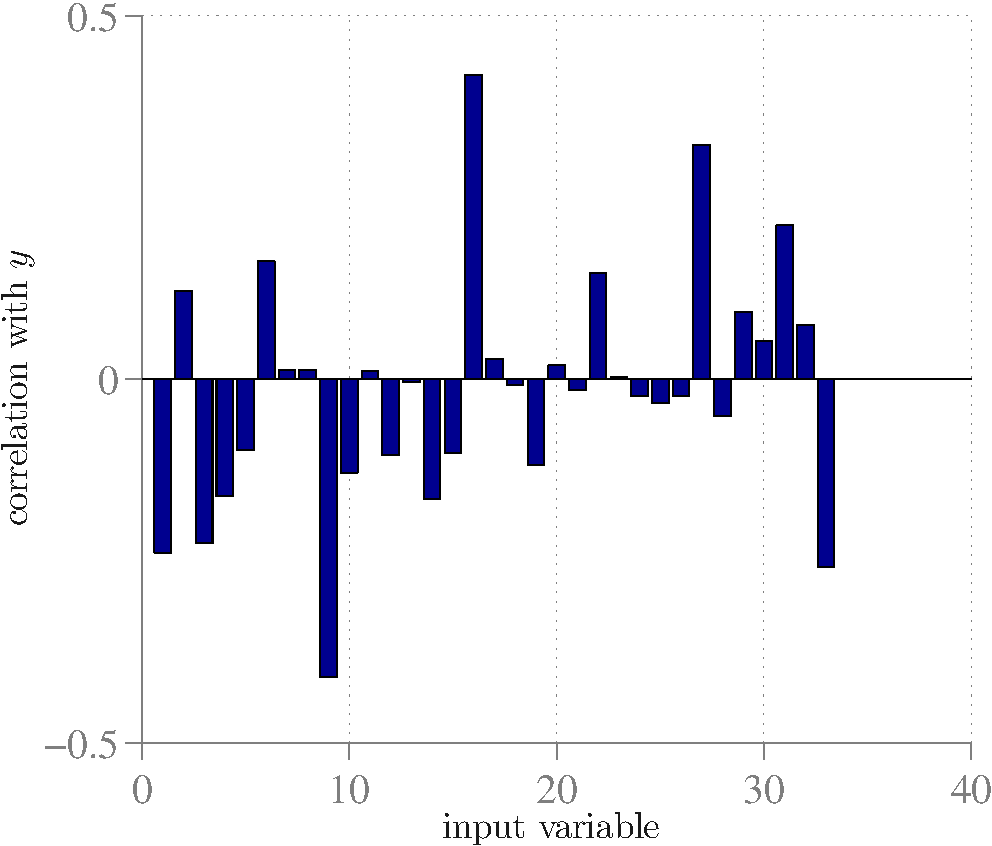
\includegraphics[width=2.5in]{../figures/bar_ycorrelation-crop.pdf} \label{fig:correlation}}
\hfill
\subfigure[Data transformation using PCA. Big correlation of some input variables with $y$ is lost.]{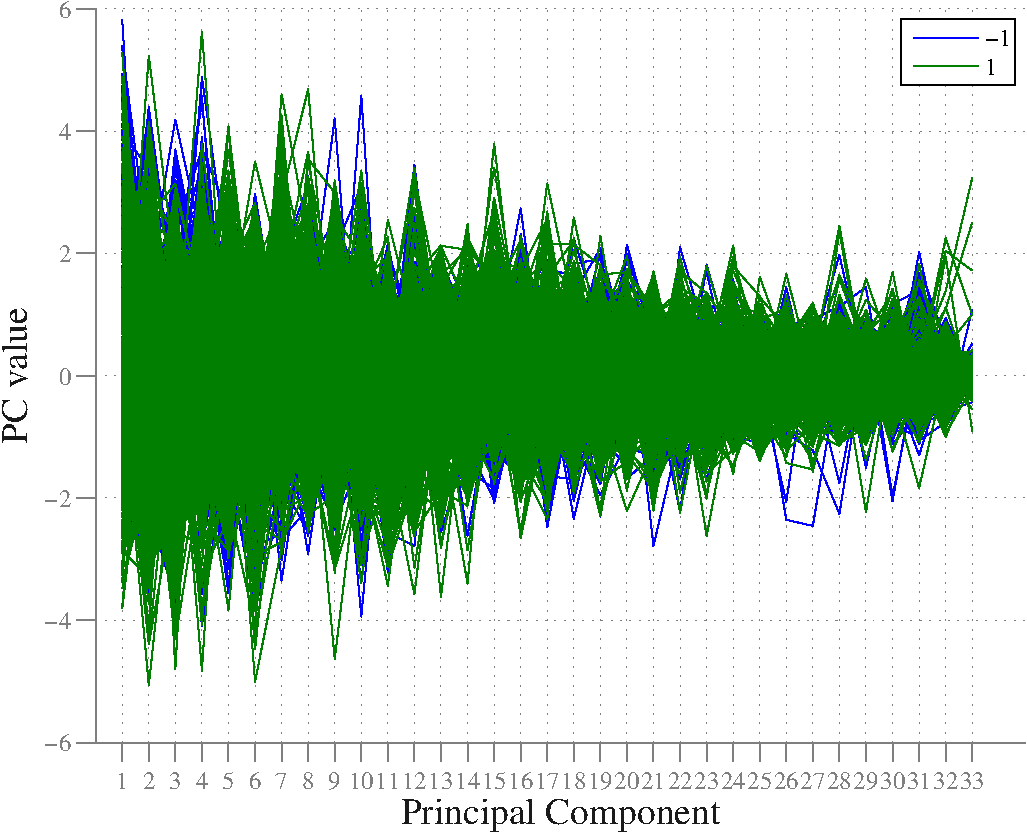
\includegraphics[width=2.5in]{../figures/parallelcoords-pca-crop.pdf} \label{fig:pca}}
\caption{}
\end{figure}

\end{subsection}
\begin{subsection}{Predicting models}
\begin{subsubsection}{Logistic regression using gradient descent}
First model we tried to fit was simple logistic regression (using Newton's method with Hessian). As we had problems with converging it for when using all input variables, we decided to try to fit it using only $9$-th input variable (the one with biggest correlation with output). 

Unfortunately even in this setting algorithm did not converge (figure \ref{fig:gdGradient}), because it tried to fit vertical line ($\beta_1$ was going to infinity), but the found model provided reasonable predictions (fig. \ref{fig:gdPrediction}).
\begin{figure}[!t]
\center

\subfigure[Prediction of output variable based only on $9$-th input variable.]{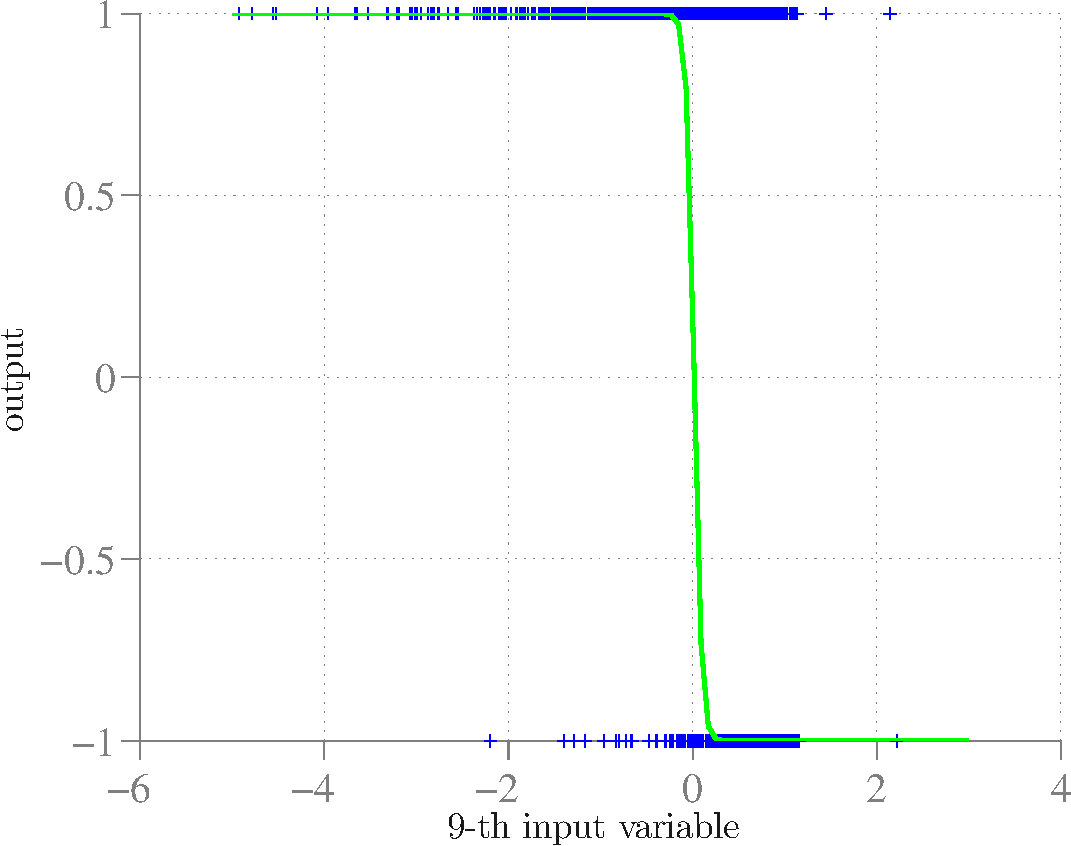
\includegraphics[width=2.5in]{../figures/gd-prediction-crop.pdf} \label{fig:gdPrediction}}
\hfill
\subfigure[Gradient norm in unpenalized gradient descent. Algorithm does not converge.]{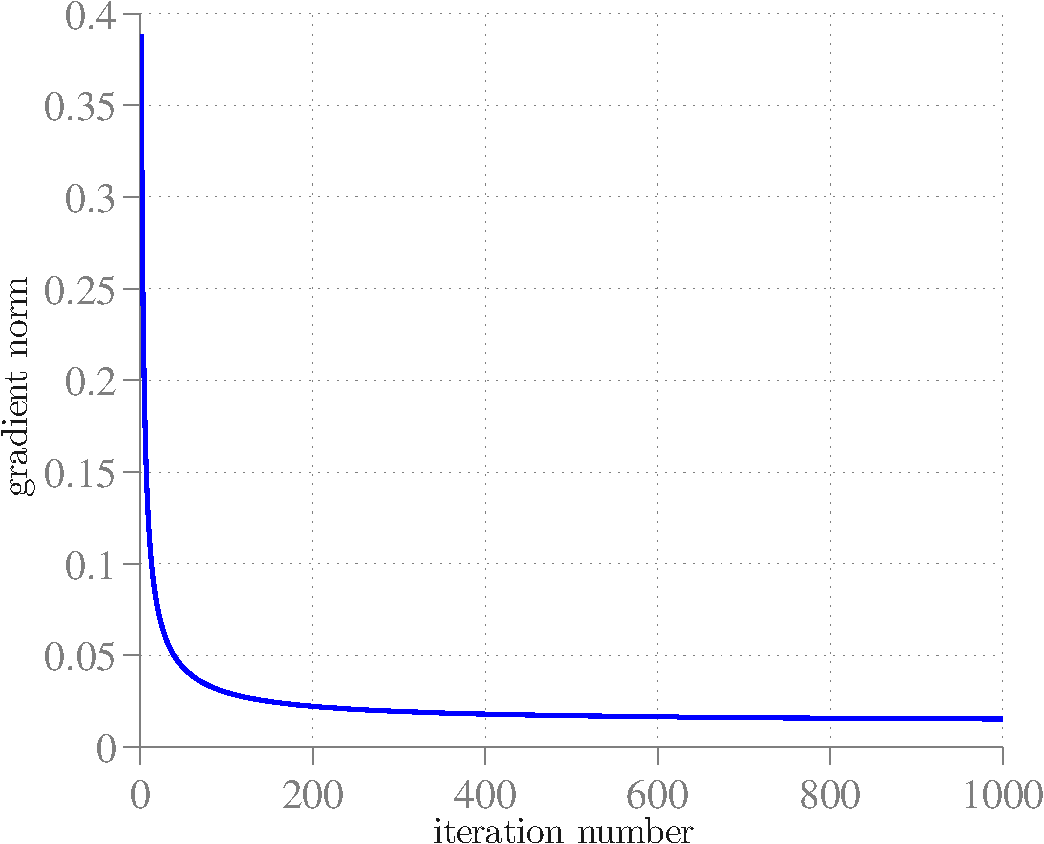
\includegraphics[width=2.5in]{../figures/gradient9-crop.pdf} \label{fig:gdGradient}}
\caption{}
\end{figure}
\end{subsubsection}
\begin{subsubsection}{Penalized logistic regression}

\end{subsubsection}
\begin{subsubsection}{SVM?}
\end{subsubsection}
\end{subsection}
\end{section}

\begin{section}{Regresssion}
\end{section}

\end{document}
